\documentclass[a4paper,11.5pt]{article}
\usepackage[textwidth=170mm, textheight=230mm, inner=20mm, top=20mm, bottom=30mm]{geometry}
\usepackage[normalem]{ulem}
\usepackage[utf8]{inputenc}
\usepackage[T1]{fontenc}
\PassOptionsToPackage{defaults=hu-min}{magyar.ldf}
\usepackage[magyar]{babel}
\usepackage{amsmath, amsthm,amssymb,paralist,array, ellipsis, graphicx,float}
%\usepackage{marvosym}

\makeatletter
\renewcommand*{\mathellipsis}{%
	\mathinner{%
		\kern\ellipsisbeforegap%
		{\ldotp}\kern\ellipsisgap%
		{\ldotp}\kern\ellipsisgap%
		{\ldotp}\kern\ellipsisaftergap%
	}%
}
\renewcommand*{\dotsb@}{%
	\mathinner{%
		\kern\ellipsisbeforegap%
		{\cdotp}\kern\ellipsisgap%
		{\cdotp}\kern\ellipsisgap%
		{\cdotp}\kern\ellipsisaftergap%
	}%
}
\renewcommand*{\@cdots}{%
	\mathinner{%
		\kern\ellipsisbeforegap%
		{\cdotp}\kern\ellipsisgap%
		{\cdotp}\kern\ellipsisgap%
		{\cdotp}\kern\ellipsisaftergap%
	}%
}
\renewcommand*{\ellipsis@default}{%
	\ellipsis@before
	\kern\ellipsisbeforegap
	.\kern\ellipsisgap
	.\kern\ellipsisgap
	.\kern\ellipsisgap
	\ellipsis@after\relax}
\renewcommand*{\ellipsis@centered}{%
	\ellipsis@before
	\kern\ellipsisbeforegap
	.\kern\ellipsisgap
	.\kern\ellipsisgap
	.\kern\ellipsisaftergap
	\ellipsis@after\relax}
\AtBeginDocument{%
	\DeclareRobustCommand*{\dots}{%
		\ifmmode\@xp\mdots@\else\@xp\textellipsis\fi}}
\def\ellipsisgap{.1em}
\def\ellipsisbeforegap{.05em}
\def\ellipsisaftergap{.05em}
\makeatother

\usepackage{hyperref}
\hypersetup{
	colorlinks = true	
}

\begin{document}
	%%%%%%%%%%%RÖVIDÍTÉSEK%%%%%%%%%%
	\setlength\parindent{0pt}
	\def\s{\hspace{0.2mm}\vphantom{\beta}}
	\def\Z{\mathbb{Z}}
	\def\Q{\mathbb{Q}}
	\def\R{\mathbb{R}}
	\def\C{\mathbb{C}}
	\def\N{\mathbb{N}}
	\def\Ra{\overline{\mathbb{R}}}
	
	\def\sume{\displaystyle\sum_{n=1}^{+\infty}}
	\def\sumn{\displaystyle\sum_{n=0}^{+\infty}}
	
	\def\narrow{\underset{n\rightarrow+\infty}{\longrightarrow}}
	\def\limn{\displaystyle\lim_{n\to +\infty}}
	\def\limx{\displaystyle\lim_{x\to +\infty}}
	
	\theoremstyle{definition}
	\newtheorem{theorem}{Tétel}[subsection] 
	
	\theoremstyle{definition}
	\newtheorem{definition}[theorem]{Definíció} 
	\newtheorem{example}[theorem]{Példa} 
	\newtheorem{task}[theorem]{Feladat} 
	\newtheorem{note}[theorem]{Megjegyzés}
	\newtheorem{revision}[theorem]{Emlékeztető}
	%%%%%%%%%%%%%%%%%%%%%%%%%%%%%%%%%%%%%%%%%%%%%%%%%%%%%%%%%%%%%%%%%%%%%
	\begin{center}
		{\LARGE\textbf{Analízis II.}}
		
		{\Large Előadás jegyzet}
		
		4. óra.
	\end{center}
	A jegyzetet \textsc{Umann} Kristóf készítette Dr. \textsc{Szili} László  előadásán. (\today)
	
	Külön köszönet jár \textsc{Csonka} Szilviának a képek elkészítésért.
	\bigskip
	
	Tantárgyi honlap: \url{http://numanal.inf.elte.hu/~szili/Oktatas/An2_BSc_2016/index_An2_2016.htm}
	
	
	\section{Folytatás.}
	\begin{revision}
		A derivált motivációja.
	\end{revision}
	\subsection{A derivált fogalma}
	\begin{note}
		A deriváltat az értelmezési tartomány belső pontjaiban értelmezzük.
	\end{note}
	\begin{definition}
		$0\not=A\subset \R$ halmaz \textbf{belső pontja} $a\in A$, ha
		\[  \exists K(a):\quad K(a)\subset A. \]
		Jele:\quad int$ A:=\{ a\in A\ | \ a $ belső pontja $A$-nak \}
	\end{definition}
	\begin{example}
		$A:=[0,1],$ \quad int$A=(0,1)$
	\end{example}
	\begin{example}
		$A:=(0,1],\quad $ int$A=(0,1)$
	\end{example}
	\begin{example}
		$A:=\{1,4,e\},\quad $int$A=\emptyset$
	\end{example}
	\begin{definition}
		$f\in\R\to\R, \quad a\in$int$\mathcal{D}_f$. $f$ \textbf{differenciálható}, vagy \textbf{deriválható} az $a$ pontban, ha
		\[ \exists\text{\quad és véges\quad }\lim_{h\to0}\frac{f(a+h)-f(a)}{h}=:f'(a)\quad \text{határérték.} \]
		$f'(a)$: $f$ \textbf{deriváltja}, vagy \textbf{differenciálhányadosa}.
		Jelöljük így is: $f\in D\{a\}$.
	\end{definition}
	\begin{note}
		$a+h=x$
		\[ f'(a)=\lim_{h\to0}\frac{f(a+h)-f(a)}{h}=\lim_{x\to a}\frac{f(x)-f(a)}{x-a} \]
	\end{note}
	\begin{note}
		 $ \varDelta_af(x):=\frac{f(x)-f(a)}{x-a}:$\quad az $f$ függvény $a$-hoz tart. \textbf{Különbségihányados}-fv, vagy \textbf{differenciahányados} függvény.
	\end{note}
	\begin{note}
		Ez a határérték mindig $\frac{0}{0}$ típusú kritikus határérték.
	\end{note}
	\begin{note}
		A differenciálhatóság ,,erősebb'' megkötés a folytonosságnak.
	\end{note}
	\begin{theorem}
		(A folytonosság és a deriválás kapcsolata)
		
		Tegyük fel, hogy $f\in\R\to\R, \quad a\in$int$\mathcal{D}_f$.
		\begin{enumerate}
			\item $f\in D\{a\}\quad \Rightarrow \quad f\in C\{a\}$.
			\item $f\in D\{a\}\quad \not\Leftarrow \quad f\in C\{a\}$.
		\end{enumerate}
		\textit{Bizonyítás:}
		\fbox{$\Rightarrow$}
		\[ f\in D\{a\}\quad \Rightarrow\quad \lim_{x-a}(f(x)-f(a))=\lim_{x\to a}\left(\frac{f(x)-f(a)}{x-a}\cdot(x-a)\right)=f'(a).\quad 0=0\quad \blacksquare \]
		\fbox{$\not\Leftarrow$} abs$\notin D\{a\}:$
		\[\frac{|x|-|0|}{x}=\left\{\begin{gathered}
		1,\quad x>0\\
		-1,\quad x<0
		\end{gathered}\right.\quad  \Rightarrow\quad \nexists\lim_{x\to 0}\frac{|x|-|0|}{x}\quad \Rightarrow\quad \text{abs}\notin\text{D}\{0\}.\quad \blacksquare \]
	\end{theorem}
	\subsection{Egyoldali deriváltak}
	\begin{definition}
		$f\in\R\to\R,\quad a\in\mathcal{D}_f$, és tegyük fel, hogy $\exists\delta>0:\quad [a,a+\delta)\subset\mathcal{D}_f.$ Ha $\exists$ és véges a $\displaystyle \lim_{x\to a+0}\frac{f(x)-f(a)}{x-a}$ hátérérték, akkor az $f$ függvény \textbf{jobbról deriválható} az $a$-ban.
		\[\displaystyle \lim_{x\to a+0}\frac{f(x)-f(a)}{x-a} =:f'_+(a) \quad \text{az $f$ jobb oldali deriváltja az $a$-ban.} \]
	\end{definition}
	\begin{note}
		A bal oldali derivált hasonló. Jele: $f'_-(a)$.
	\end{note}
	\begin{note}
		$f$ deriválható az $a$-ban $\quad\Leftrightarrow \exists f'_+(a), \quad \exists f'_-(a)$, \quad és\quad  $ f'_+(a)=f'_-(a).$ \quad Jele:\quad $f'(a).$
	\end{note}
	\subsection{Deriváltfüggvény.}
	\begin{definition}
		Ha $f\in\R\to\R$, és 
		\[ \{ a\in\text{int}\mathcal{D}_f \ |\ f\in D\{a\} \}\not=\emptyset, \]
		akkor
		\[ f':\quad \{ a\in\text{int}\mathcal{D}_f \ |\ f\in D\{a\} \}\to\R,\quad x\to f'(x) \]
		az $f$ \textbf{deriváltfüggvénye}, vagy \textbf{differenciálhányados-függvénye}.
	\end{definition}
	\subsection{Elemi függvények deriváltja.}
	\begin{note}
		Lásd: honlapon táblázat.
	\end{note}
	\begin{enumerate}
		\item Konstansfüggvény: $c\in \R$ rögzített,\quad  $f(x)=c.\quad (x\in\R)$
		\[ \forall x\in\R:\quad f\in D\{x\}\quad \text{és}\quad f'(x)=0,\quad \fbox{(c)'=0}. \]
		\item Hatványfüggvények: $n\in\N, \quad f(x):=x^n\quad (x\in\R)$.
		\[ \forall x \in\R,\quad f\in D\{x\},\quad \text{és}\quad (x^n)'=n\cdot x^{n-1}\quad (x\in\R) \]
		
		\textit{Bizonyítás:} 
		\[ \frac{f(x+h)-f(x)}{h}=\frac{(x+h)^n-x^n}{h}\quad \overset{\frac{0}{0}}{=}\quad \frac{h\cdot[(x+h)^{n-1}+\ldots+x^{n-1}]}{h}\quad \underset{h\to0}{\longrightarrow}\quad n\cdot x^{n-1}\quad \blacksquare \]
		\item Reciprok függvény: $f(x):=\frac{1}{x}\quad (x\in\R\setminus\{0\})$
		\[ \forall x\in\R\setminus\{0\}\quad \Rightarrow\quad f\in D\{x\}\quad \text{és}\quad \left(\frac{1}{x}\right)'=-\frac{1}{x^2}\quad (x\in\R\setminus\{0\}) \]
		\item abs$\notin D\{0\}.$
		\item Négyzetgyökfüggvény. $f(x):=\sqrt{x}\quad (x\in[0,+\infty[)$
		\[ \forall x>0\text{-ra}: \quad f\in D\{x\}:\quad (\sqrt{x})'=\frac{1}{2\sqrt{x}}\quad (x\in(0,+\infty)) \]
		\item $\sin$
		\[ \sin'x=cosx\quad (x\in\R) \]
		
		\textit{(biz nélkül.)}
		\item $\cos$\[ \cos'x=-sin\quad (x\in\R) \]
		
		\textit{(biz nélkül.)}
	\end{enumerate}
	\subsection{Ekvivalens átfogalmazás (lineáris közelítés). Érintő.}
	\begin{theorem}
		(Lineáris közelítés)
		
		Tegyük fel, hogy $f\in\R\to\R,\quad a\in$int$\mathcal{D}_f$
		\[ f\in D\{a\}\quad \Leftrightarrow\quad 
		\left\{\begin{gathered}
		\exists A\in\R\quad \text{és}\quad \exists \varepsilon:\quad \mathcal{D}_f\to\R,\quad \lim_a\varepsilon=0\\
		f(x)-f(a)=A(x-a)+\varepsilon(x)(x-a)\quad (x\in\mathcal{D}_f)
		\end{gathered}\right. \]
		$A=F'(a)$.
		\medskip
		
		\textit{Bizonyítás:}
		
		\fbox{$\Rightarrow$}
		\[ f\in D\{a\}\quad \Rightarrow\quad \lim_{x\to a}\frac{f(x)-f(a)}{x-a}=f'(a)\quad \Rightarrow\quad \lim_{x\to a}\underbrace{\left(\frac{f(x)-f(a)}{x-a}-f'(a)\right)}_{=:\varepsilon(x)}=0 \]
		Így: \quad $\lim_a\varepsilon=0$, és 
		\[f(x)-f(a)=f'(a)(x-a)+\varepsilon(x)(x-a)\quad (x\in\mathcal{D}_f)\checkmark  \]
		\fbox{$\Leftarrow$} Tegyük fel, hogy $\exists A\in\R,\quad \exists \varepsilon:\quad \mathcal{D}_f\to\R,\quad \lim_a\varepsilon=0:$
		\[ f(x)-f(a)=A(x-a)+\varepsilon(x)(x-a)\quad \overset{x\not=a}{\Rightarrow}\quad \underbrace{\frac{f(x)-f(a)}{x-a}}_{\overset{x\to a}{\longrightarrow}f'(a)}=\underbrace{A+\varepsilon(x)}_{\overset{x\to a}{\longrightarrow}A} \]
		\[ \Rightarrow f'(a)=A\quad \blacksquare \]
	\end{theorem}
	\begin{note}
		Szemléletes jelentése.
		
		$f\in D\{a\}$.
		\begin{figure}[H]
			\centering
			%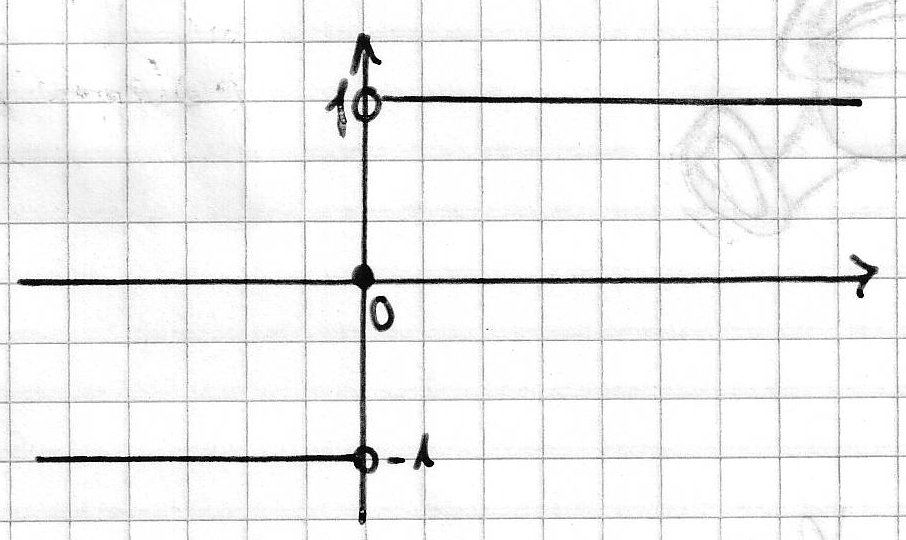
\includegraphics[height=3cm]{kepek/2_abra_signum.jpg}
			\caption{}\label{}
		\end{figure}
		\[ f(x)-f(a)=\underbrace{A(x-a)}_{\text{\textbf{Főrész}}}\quad \quad +\underbrace{\varepsilon(x)(x-a)}_{\text{sokkal kisebb. \textbf{Maradék}}} \]
		ha $x\sim a\quad \underset{\lim_a\varepsilon>0}{\Rightarrow}\quad f\in D\{a\}\quad \Rightarrow\quad f(x)-f(a)\sim A(x-a).\quad \blacksquare$ 
	\end{note}
	\begin{note}
		$f'(a)$ definíció általánosítsa $\to$ nem mindig.
		lin. köz általánosítása $\to$ gyakran problémamentes. $\blacksquare$
	\end{note}
	\begin{revision}
		Érintő: $f\in D\{a\}$
		\begin{figure}[H]
			\centering
			%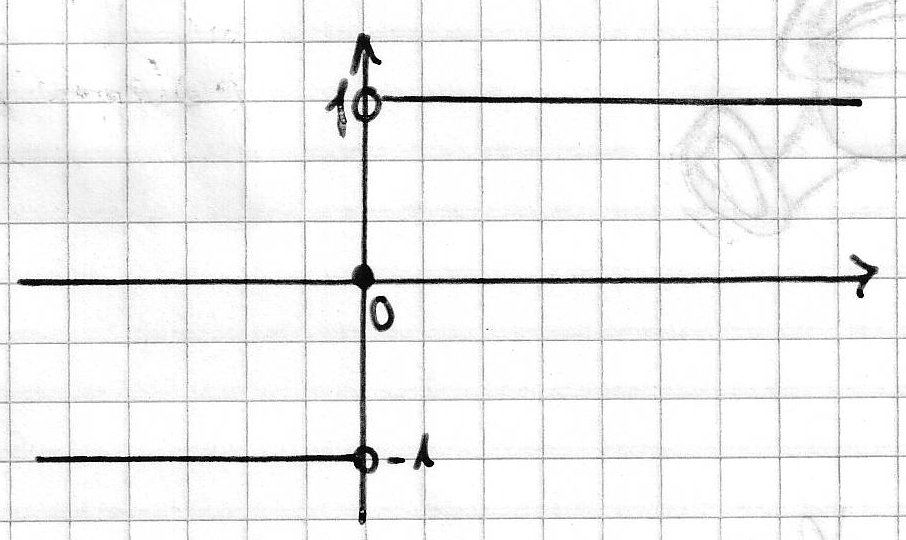
\includegraphics[height=3cm]{kepek/2_abra_signum.jpg}
			\caption{}\label{}
		\end{figure}
	\end{revision}
	\begin{definition}
		$f:\R\to\R$ függvény grafikonjának van érintője, az $(a,f(a))$ pontban, ha $f\in D\{a\}$.
		
		\smallskip
		A grafikon $(a,f(a))$-béli \textbf{érintője} az
		\[ x=f'(a)(x-a)+f(a) \]
		egyenletű egyenes.
	\end{definition}
	\begin{note}
		HF: Kör, parabola érintője a fenti definícióból; ez ekvivalens a középiskolai definícióval.
	\end{note}
\end{document}
